\documentclass[10pt]{article}
\usepackage[margin=0.72in]{geometry}
\usepackage{amsmath,amssymb}
\usepackage{booktabs}
\usepackage{enumitem}
\usepackage{graphicx}
\usepackage{xcolor}
\usepackage[colorlinks=true,linkcolor=black,urlcolor=black]{hyperref}
\setlength{\parindent}{0pt}
\setlength{\parskip}{3.2pt}
\pagestyle{empty}

\newcommand{\hd}[1]{\vspace{2pt}\textbf{\large #1}\vspace{1pt}\\}

\begin{document}

{\LARGE\textbf{UVLO Lock-Out Latch for an LM5176 Buck-Boost}}\\[2pt]
{\small USB-C PD $\to$ 12\,V fan-array controller, 42\,W --- design summary.
Full derivations: \texttt{uvlo\_tlv431.pdf} (divider), \texttt{uvlo\_latch.pdf}
(latch). Schematic overleaf.}

\vspace{4pt}\hrule\vspace{5pt}

\hd{Problem}
The control loop is deliberately slow --- its crossover sits far below the
$\sim$160\,Hz commutation pulses of the fan load, so the loop does not chase
them and the output bank absorbs them instead. With that loop, the LM5176's
pre-biased startup does not survive a brief input dropout: on recovery the
part restarts into a still-charged output and misbehaves. TI support could not
root-cause it and proposed raising the crossover frequency --- precluded by the
very requirement that set the low crossover in the first place.

\hd{Approach}
A discrete lock-out latch (four BJTs + a TLV431 shunt reference, all jellybean
parts) supplied from $V_{OUT}$ rather than $V_{IN}$. The TLV431 watches the
EN/UVLO divider; when the \emph{input} sags the reference stops conducting, an
actively driven ``dearm'' transistor releases, and a two-transistor SCR core
fires and clamps EN/UVLO low. Because the latch is powered from the
\emph{output}, it holds until $V_{OUT}$ has decayed to $\approx$1.1\,V --- so
every restart begins from a dead output and the pre-bias path is never
exercised. Cold start is safe by construction: at $V_{OUT}=0$ the latch is
unpowered.

\hd{Result} (worst case over $\pm3\%$ resistors, full datasheet spreads, 0--50\,\textdegree C)

\vspace{-3pt}
The two rails carry independent threshold sets --- input thresholds decide
\emph{when the converter runs and when the latch trips}; output thresholds
decide \emph{when the latch is able to act at all}, since $V_{OUT}$ is its supply.

\vspace{-4pt}
\begin{center}\small
\begin{tabular}{@{}p{0.17\textwidth}p{0.36\textwidth}p{0.42\textwidth}@{}}
\toprule
\textbf{$V_{IN}$ domain} & divider $R_2/R_{1a}/R_{1b}=420/150/15\,\mathrm{k}\Omega$
  & turn-on guaranteed in \textbf{2.75--4.49\,V}; latch trips at
    $V_{IN}\approx3.5$\,V, inside the IC's own hysteresis window \\[3pt]
\textbf{$V_{OUT}$ domain} & latch arms above \textbf{2.8\,V} nom.\
  (2.0--3.6\,V worst case) & dearm circuit active from \textbf{2.05\,V};
  EN released once $V_{OUT}$ falls to 1.0--1.8\,V \\[3pt]
\textbf{Cost} & 6.9\,mA from the 12\,V rail & every resistor a stocked JLCPCB
  basic 0603 part \\
\bottomrule
\end{tabular}
\end{center}

\vspace{-3pt}
The divider was chosen to push the \emph{earliest} possible turn-on as high as
it will go (2.75\,V) while the \emph{latest} still clears a sagging 4.5\,V USB
rail --- a two-sided constraint on the same ratio, not a single target.

\hd{Engineering notes --- where the work actually went}
\begin{itemize}[leftmargin=1.1em,itemsep=2pt,topsep=1pt]
\item \textbf{Correlated vs.\ independent worst case.} Comparing the
  \emph{population bands} of the three $V_{IN}$ threshold events makes the
  design look infeasible. But the latch trip and the IC's own dropout are
  events of the same device at the same instant: $I_{STBY}$, $I_{HYS}$,
  $V_{IN}$ and $R_2$ cancel in the difference, leaving a gap set only by
  $V_{TLV}$, the divider ratio and $V_{th}$. Differencing per unit rather than
  per band is what makes a solution exist at all.
\item \textbf{A device model that is traceable, not assumed.} No $V_{BE}$ spec
  exists at the tens-of-\textmu A the latch runs at, so the datasheet
  $V_{BE(\mathrm{sat})}$ box (0.65--0.85\,V at 10\,mA) is scaled by
  $V_T\ln(I_1/I_2)$ down to 0.50--0.70\,V at 30\,\textmu A. Every threshold is
  then guaranteed by spec limits alone --- no unit screening, no reliance on
  typicals.
\item \textbf{Design against a physics floor (an output-rail limit).} The dearm
  transistor draws its base current from $V_{OUT}$ through the TLV431, so it
  cannot turn on until $V_{OUT}\ge V_{KA}^{\max}+V_{EB}=2.02$\,V --- a hard
  limit, independent of resistor choice. The design sits at 2.05\,V, 27\,mV
  above it, which is what keeps the latch's arm point low and the unprotected
  output band as narrow as the parts allow.
\item \textbf{A vendor constraint found on paper, not in smoke.} While latched,
  the reference's cathode floats to $\approx$15.4\,V. A 6\,V-rated TLV431 (TI)
  would sit outside its absolute maximum during normal operation of this
  circuit; the pin-compatible onsemi part (16\,V) is what the design assumes.
  The same excursion shifts the reference minimum by 21\,mV --- enough to
  invalidate an earlier resistor triple that had passed.
\item \textbf{A revision scrapped on analysis.} The first latch used
  sub-threshold leakage as its trigger. That current is unspecified and spans
  $\sim2000\times$ over part spread and temperature, so it was replaced by a
  trigger defined purely by resistor ratios and spec'd $V_{BE}$.
\end{itemize}

\hd{Verification}
Two Python tools: closed-form constraint geometry plus an exhaustive corner
sweep over stocked part values, emitting \textbf{21 pass/fail checks} (0 fail;
2 flagged as bench-review items) and the constraint-region figures. Every
threshold is cross-checked against an LTspice transient --- simulated engage
\textbf{3.47\,V vs.\ 3.51\,V predicted (1.3\,\%)}, hold through a full input
re-application at $V_{OUT}=12$\,V, release at $V_{OUT}=1.08$\,V inside the
predicted 1.0--1.8\,V band. The checker re-reads the \texttt{.raw} file, so the
simulation and the hand analysis cannot silently drift apart.

\hd{Known limit, and the open question it leaves}
The latch can only act once $V_{OUT}$ is above its arm point, so \textbf{a
dropout with $V_{OUT}$ anywhere below $\approx$3.6\,V (worst-case unit) is
unprotected} --- the band runs down to zero, not just to the release point.
Two things follow, and the second is not yet closed:
\begin{itemize}[leftmargin=1.1em,itemsep=2pt,topsep=1pt]
\item Body diodes do \emph{not} bound the exposure: the converter switches
  synchronously, so an enabled FET conducts either way.
\item The right failure model is \emph{energy}, not charge, and it is not
  benign. A passive dump through a conducting FET would merely equalise the two
  banks at 3.56\,V. But a buck-boost moves energy through an inductor, and the
  input bank is 90$\times$ smaller ($C_{OUT}\approx18.9$\,mF vs.\
  $C_{IN}\approx0.21$\,mF), so a reverse transfer is a \emph{boost} into a
  small capacitor:
  \[
  V_{IN}\;\approx\;V_{OUT}\sqrt{C_{OUT}/C_{IN}}\;=\;3.6\times9.5\;\approx\;
  \mathbf{34\ V},
  \]
  against a 22\,V operating maximum and 35\,V input electrolytics --- and
  whatever USB source is attached sees it. Even a quarter of the energy
  reaching the input gives $\approx$17\,V.
\end{itemize}
\vspace{-3pt}
\textbf{Open item (safety, not housekeeping):} confirm by bench and simulation
that the LM5176's pre-biased startup performs no reverse energy transfer for
$V_{OUT}$ below the arm point. Until that is shown, the low-$V_{OUT}$ band is
an accepted, documented exposure --- and the case for extending protection
below the arm point (or clamping the input) rests on that measurement.

\vspace{3pt}\hrule\vspace{3pt}
{\small\textbf{Artifacts:} \texttt{10a\_uvlo\_resistor\_search.py} (divider
search) $\cdot$ \texttt{10b\_uvlo\_latch.py} (latch checks + LTspice
cross-check) $\cdot$ two LaTeX design notes $\cdot$ LTspice schematic and
transient.}

\newpage

{\large\textbf{Circuit}}\\[2pt]
{\small Left: the lock-out latch, supplied from $V_{OUT}$. Right: the LM5176
\texttt{EN/UVLO} divider ($R_2$, $R_{1b}$, $R_{1a}$) that the TLV431 senses and
that Q1 clamps, plus the behavioural source used to model the EN-pin bias
current in simulation.}

\vspace{6pt}
\begin{center}
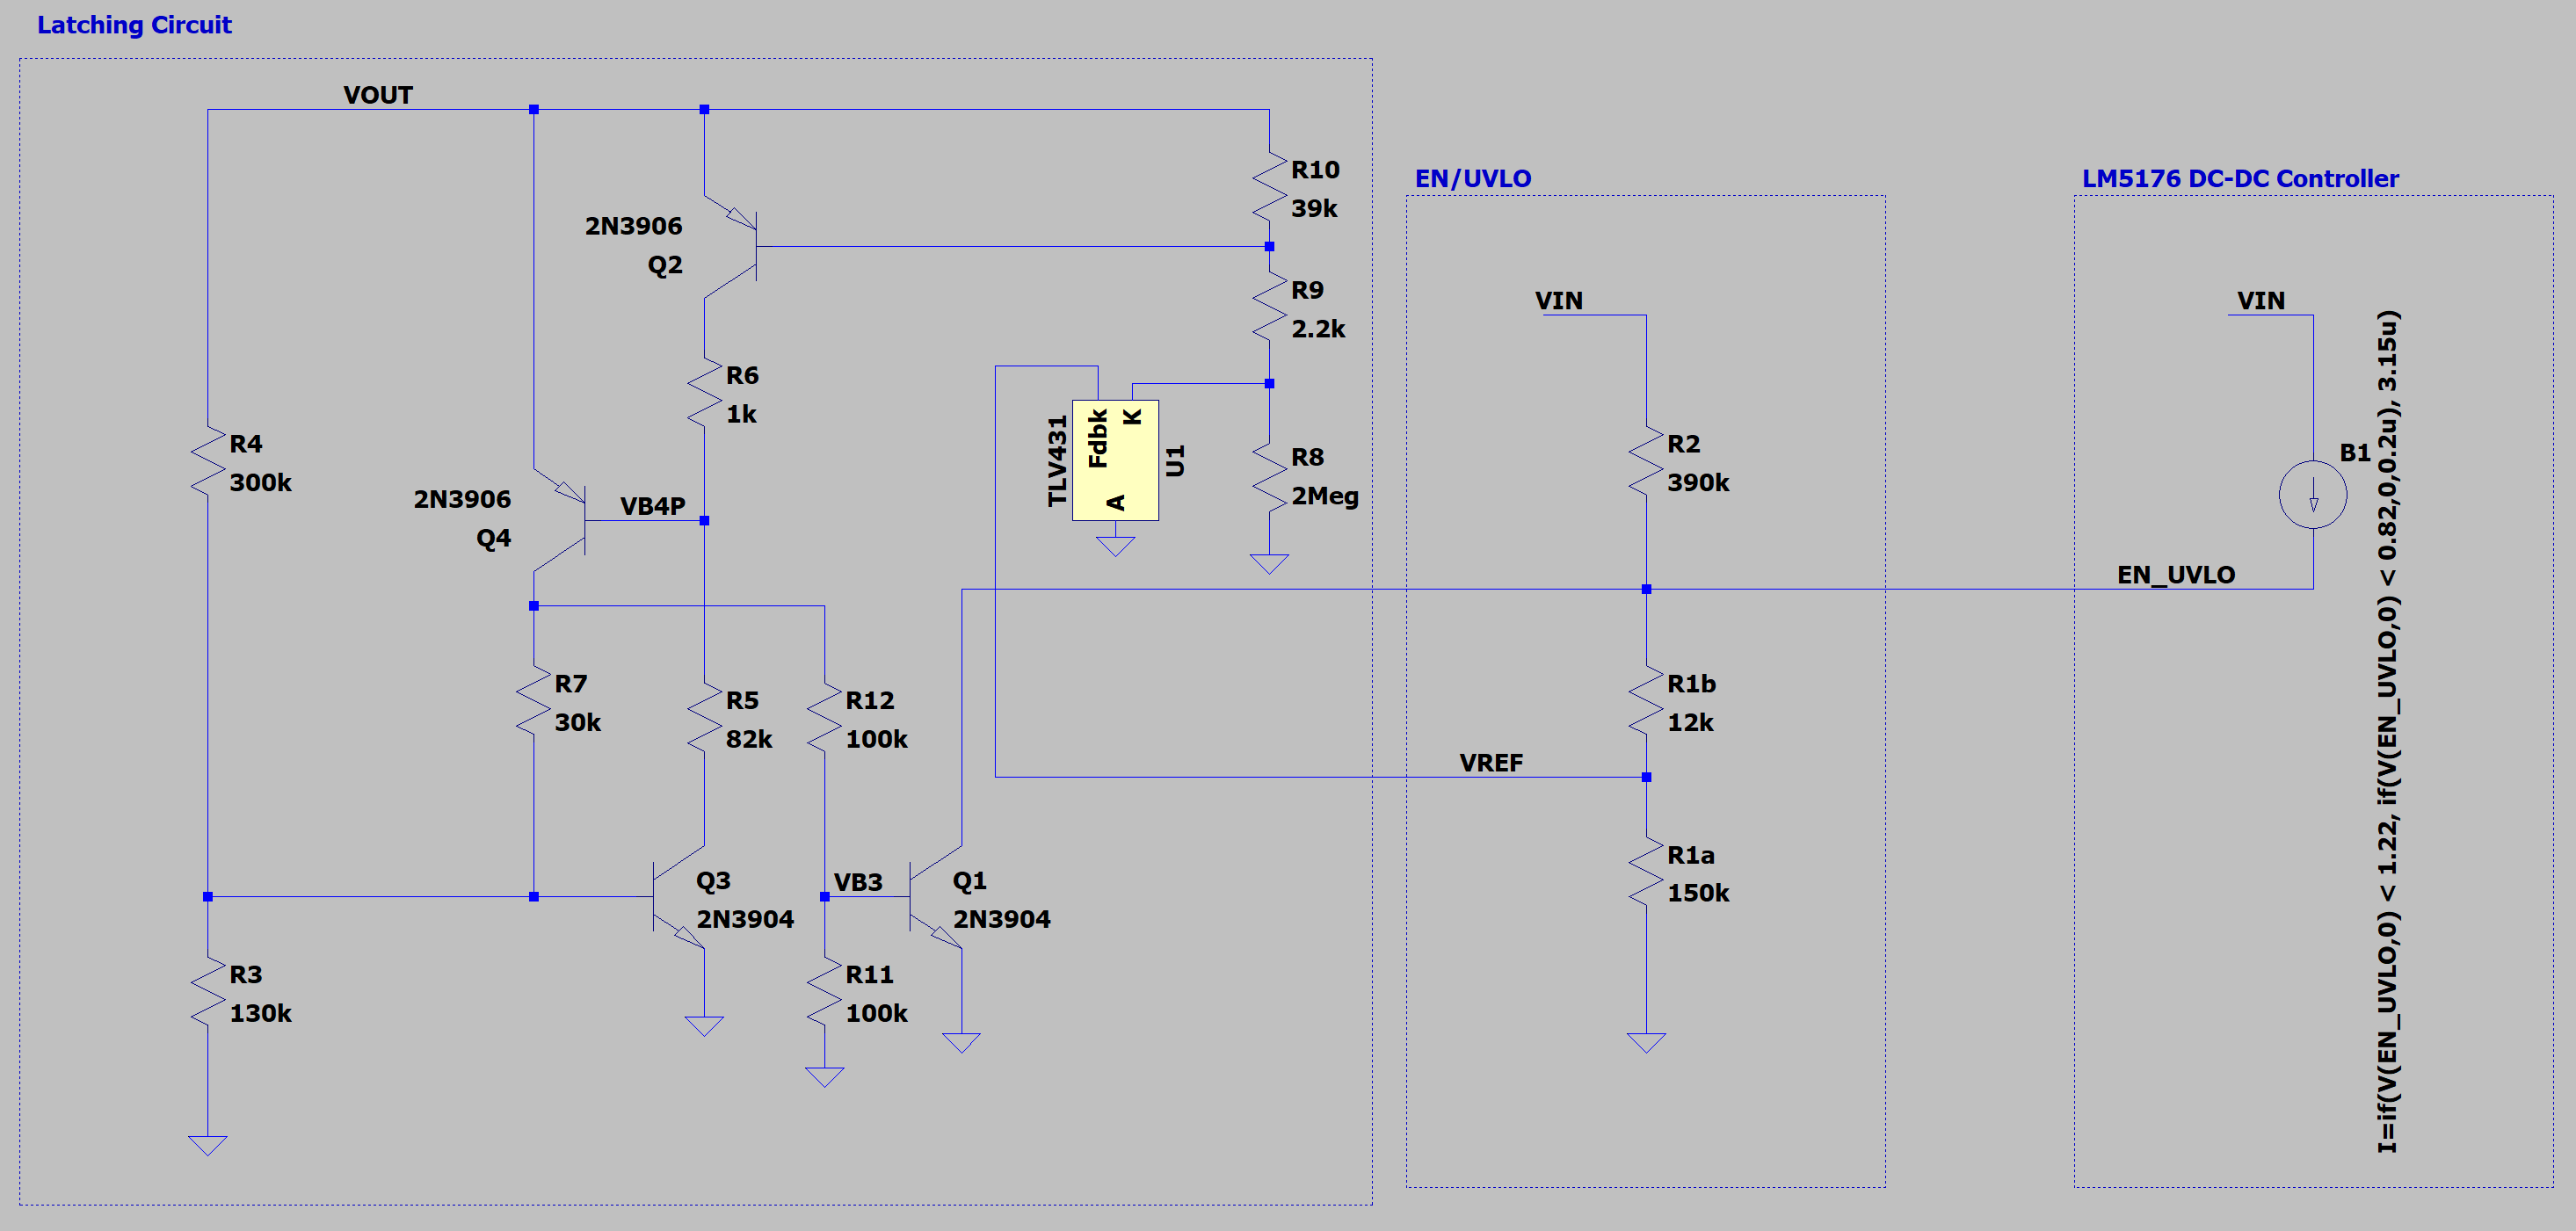
\includegraphics[width=\textwidth]{figures/divider_latch_schematic.png}
\end{center}

\vspace{4pt}
{\large\textbf{Simulated sequence}}\\[2pt]
{\small Cold start $\to$ run $\to$ input dropout (latch engages) $\to$ input
returns while $V_{OUT}$ is still high (latch holds) $\to$ $V_{OUT}$ decays
(latch releases, clean restart).}

\vspace{6pt}
\begin{center}
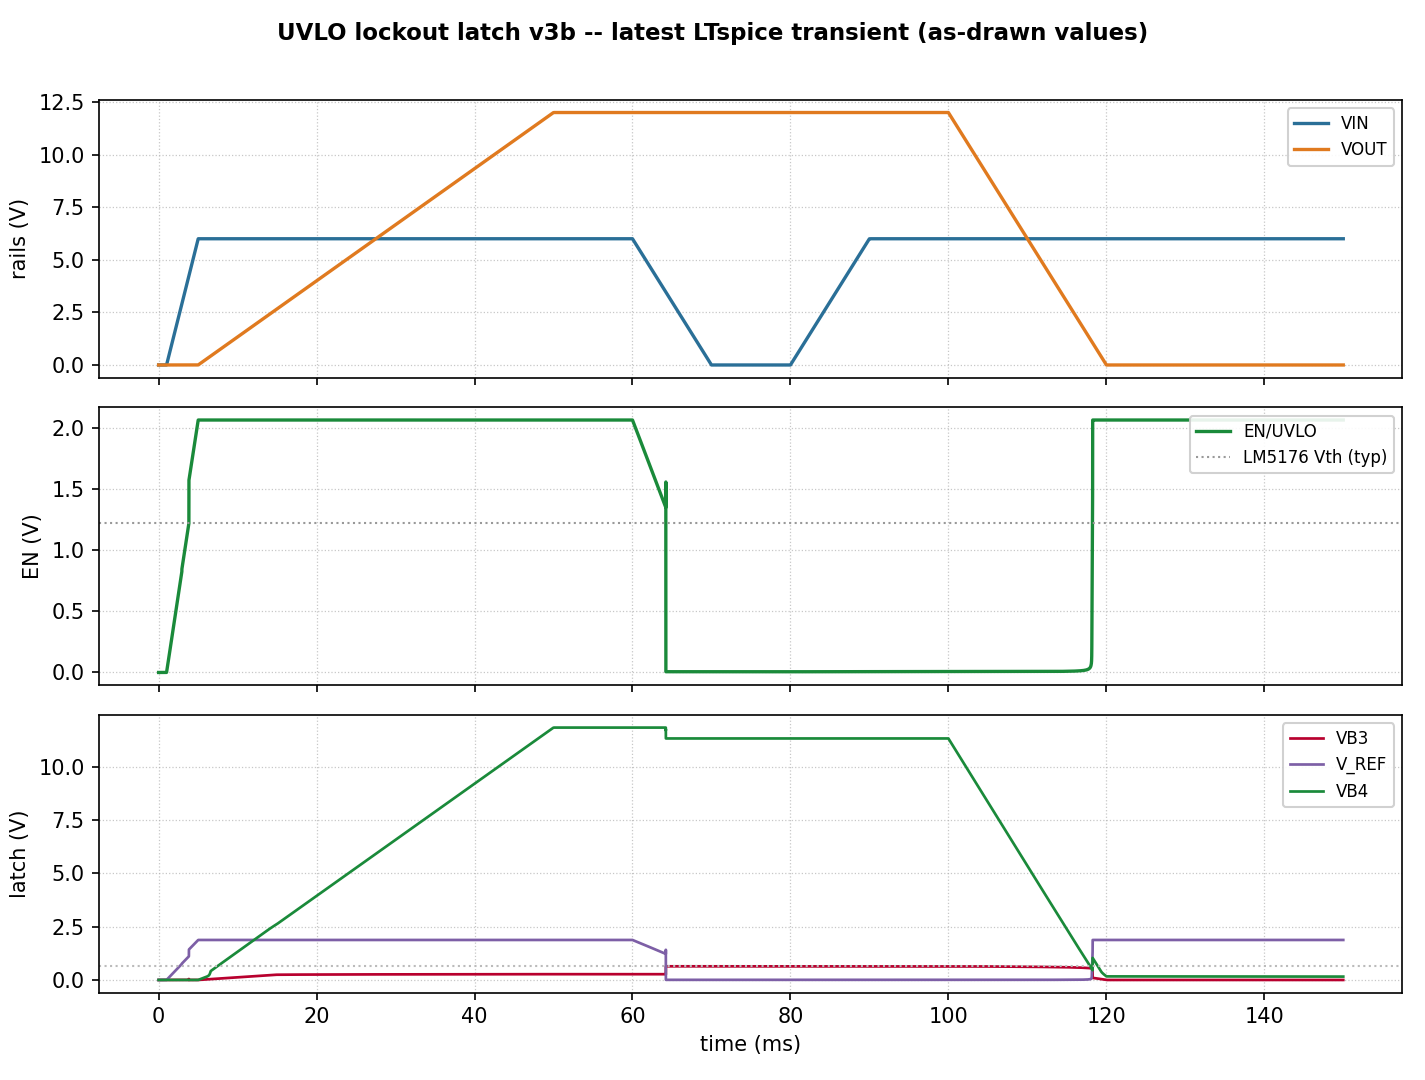
\includegraphics[width=0.92\textwidth]{figures/uvlo_latch_sim.png}
\end{center}

\end{document}
